%\section{Head Calibration System}
\section{Robot Head Model}
\label{sec:head_calibration_system}

The robot head is represented by a kinematic chain formed by multiple rotation joints serially coupled (see figure \ref{fig:head_kinematic_model_prob_form}a). 

\begin{figure}
\centering
    \centering
    \begin{tabular}{ccc}
    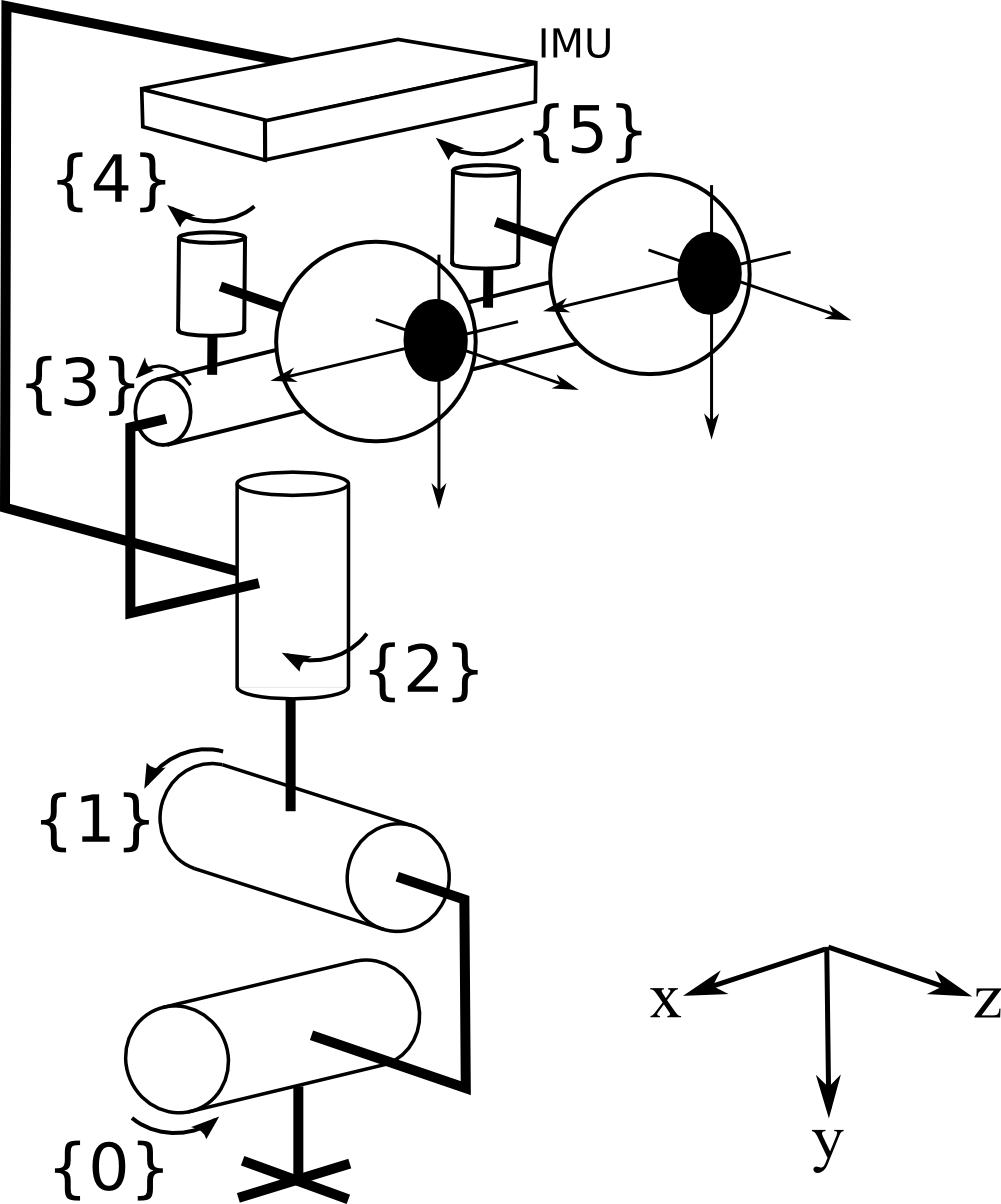
\includegraphics[width=0.3\columnwidth]{images/Head_Kinematic_Model_v2} & &
    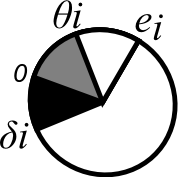
\includegraphics[width=0.15\columnwidth]{images/offset_model} \\
    a) & & b)
    \end{tabular}
    \caption{The head kinematic model; a) the corresponding serial chain of joints, from the neck base $\left\{ 0\right\} $ to the eyes final joints $\left\{ 4\right\} $ and $\left\{ 5\right\} $; b) a cross section of a joint $\left\{ i\right\} $ showing the relation between the encoder measurement $e_i$ and the offset $\delta_i$ in the calibrated joint angle $\theta_i$}
\label{fig:head_kinematic_model_prob_form}
\end{figure}

Each joint $i$ can rotate by an angle $\theta_i$ around its axis of rotation. In a calibrated internal model, $\theta_{i}$ corresponds to the exact measurement given by the encoder sensor, $e_i$. However if the internal model is not properly calibrated, there is an offset $\delta_{i}$ that must be considered and the angle $\theta_{i}$ becomes a linear combination of the encoder measurement and the offset, as seen in figure \ref{fig:head_kinematic_model_prob_form}b), with the relation given by:

\begin{equation}
\theta_{i} = e_{i}-\delta_{i}
\label{eq:offset_relation}
\end{equation}

Let $^{i+1}R_{i}\left(\theta_{i}\right)$ represent a rotation between two consecutive joints, $i$ and $i+1$. This rotation is a function of the rotation angle $\theta_{i}$ associated to the $i$th joint. The complete rotation from a reference frame $\{n\}$ to the base of the kinematic chain $\{0\}$ is written as

\begin{equation}
^{n}R_{0}\left(\theta_{0},\ldots,\theta_{n-1}\right)={}^{n}R_{n-1}\left(\theta_{n-1}\right)\ldots{}^{2}R_{1}\left(\theta_{1}\right){}^{1}R_{0}\left(\theta_{0}\right)
\label{eq:kinematic_chain}
\end{equation}

We can easily see that an offset in one of the primary joints or the composition of multiple offsets through the kinematic chain may introduce large errors in the final orientation of its end-effector. The goal of our work is to estimate all the offsets $\delta_{i}$ so the rotation given by the kinematic model adequately reflect the real state of the system and the relation (\ref{eq:offset_relation}) holds for every considered joint.

In the case of a typical robot head equipped with an IMU and stereo cameras, which includes all the head joints from the neck base $\{0\}$ to both eyes $\{4\}$ and $\{5\}$ as seen in figure \ref{fig:head_kinematic_model_prob_form}a), we want to find the offsets defining the head's absolute zero position, with both cameras pointing to the front (projection planes orthogonal to the floor) and a gravity vector reading, given by the IMU, corresponding to a vertical vector pointing down.

\subsection{Observability Analysis}

The model presented in (\ref{eq:kinematic_chain}) is able to describe any kinematic chain from a combination of multiple rotation matrices, one per each joint. However, this model presents observability problems when consecutive joints are rotating about the same rotation axis, since their rotation becomes coupled. Let's consider the following example where a kinematic chain has two consecutive joints rotating about the $x$ axis, by angles of $\alpha$ and $\beta$. 

\begin{equation}
R\left(\alpha,\beta\right)=R_{x}\left(\alpha\right)R_{x}\left(\beta\right)
\label{eq:rotation_observability}
\end{equation}
with $R_{x}\left(\alpha\right)$ given by:

\begin{equation}
R_{x}\left(\alpha\right)=\left[\begin{array}{ccc}
1 & 0 & 0\\
0 & \cos\left(\alpha\right) & -\sin\left(\alpha\right)\\
0 & \sin\left(\alpha\right) & \cos\left(\alpha\right)
\end{array}\right]
\end{equation}
(analogous for $R_{x}\left(\beta\right)$).

After the product, equation (\ref{eq:rotation_observability}) becomes:

\begin{equation}
R\left(\alpha,\beta\right)=\left[\begin{array}{ccc}
1 & 0 & 0\\
0 & \cos\left(\alpha+\beta\right) & -\sin\left(\alpha+\beta\right)\\
0 & \sin\left(\alpha+\beta\right) & \cos\left(\alpha+\beta\right)
\end{array}\right]
\end{equation}
where we applied trigonometric relations to simplify the notation. In the final rotation $R\left(\alpha,\beta\right)$, $\alpha$ and $\beta$ are coupled. Considering $\theta=\alpha+\beta$, this coupling behaviour means any value of $\theta$ can be obtained from an infinite number of linear combinations of $\alpha$ and $\beta$. Having infinite possibilities for both angles, the system can't estimate the real offsets for each joint. However, the differential between the two is always constant and by fixing one of the joints (assuming it has no offset), it is still possible estimate the offset for the other joint.

\section{Calibration Methodology}\label{sec:calibration_methodology}

The base of our calibration system is an Implicit Extended Kalman Filter (IEKF) since part of our observations' predictions can not be directly obtained from the system state only. In the following sections we will explain the IEKF in more detail and introduce the dynamic and observation models for our filter considering the nature of the problem.

\subsection{Implicit Extended Kalman Filter}

The Implicit Extended Kalman Filter (IEKF) is a variation of the Extended Kalman Filter (EKF) \cite{Ribeiro04} where the measurements take the form of an implicit constraint that is a function of both the system state and the sensors observations. Soatto introduced this variation in \cite{Soatto96,Soatto96b} as a way to estimate the motion of a moving camera using the epipolar constraint \cite{Hartley04} as the system's measurements.

\subsubsection{State and Observation Model}

In a generic IEKF the system assumes its state evolves according to a certain dynamic model (identical to the EKF's), linear or not, considering it has no inputs, as:

\begin{equation}
x^{k+1}=f^{k}\left(x^{k}\right)+w^k
\label{eq:iekf_generic_prediction}
\end{equation}
where $f^k$ corresponds to the state transition function, $x^{k}$ and $x^{k+1}$ denote the system states at time instants $k$ and $k+1$ and $w^{k}\sim \mathcal{N}\left(0,Q^{k}\right)$ is an additive zero mean Gaussian noise with covariance $Q^{k}$.

In the standard EKF the measurements are explicit functions of the system state $x$ and they can be obtained from a measurement model of the form:

\begin{equation}
y^{k+1} = h^{k+1}\left(x^{k+1}\right) + v^{k+1}
\label{eq:iekf_generic_measurement_y}
\end{equation}
where $h^{k+1}$ corresponds to the measurement function, with $v^{k+1}\sim \mathcal{N}\left(0,R^{k+1}\right)$ as an additive zero mean Gaussian noise with covariance $R^{k+1}$. However in the IEKF, the filter measurement equation takes the form of a constraint $z$ that must be fulfilled and is an implicit function of both the system state $x$ and the physical measurements from the sensors, $y$:

\begin{equation}
z^{k+1} = h^{k+1}\left(x^{k+1}, y^{k+1}\right) = 0
\label{eq:iekf_generic_constraint}
\end{equation}

This hybrid model is extremely useful when the system's innovation $z^{k+1}$ cannot be linearly obtained from the predicted observations and the real observations. \footnote{In the EKF $z^{k+1}$ is given by the difference between the predicted observations $\bar{y}^{k+1}=h^{k+1}\left(\bar{x}^{k+1}\right)$ and the real observations $y^{k+1}$, $z^{k+1}=\bar{y}^{k+1}-y^{k+1}$.}

\subsubsection{Prediction and Update Equations}

The IEKF, like the EKF, is a two-step procedure with a prediction and an update step. In the prediction step, the system state is propagated using the dynamic model described in (\ref{eq:iekf_generic_prediction}):

\begin{equation}
\bar{x}^{k+1}=f^{k}\left(\hat{x}^{k}\right)
\label{eq:iekf_generic_state_prediction}
\end{equation}
where $\hat{x}^{k}$ corresponds to the estimate of $x$ from the previous time instant, with the previous state covariance matrix estimation $\hat{P}^{k+1}$ being propagated and predicted using the standard filter equation:

\begin{equation}
\bar{P}^{k+1}=\mathcal{F}^{k}\hat{P}^{k}\left(\mathcal{F}^{k}\right)^{T}+Q^{k}
\label{eq:iekf_generic_state_cov_prediction}
\end{equation}
where $\mathcal{F}^{k}$ is the Jacobian of $f^{k}$ obtained by linearizing the function, evaluated at the previous state estimate $\hat{x}^{k}$:

\begin{equation}
\mathcal{F}^{k}=\left.\frac{\partial f^{k}}{\partial x}\right|_{x=\hat{x}^{k}}
\end{equation}

In the update step, the predicted filter measurement $\bar{z}^{k+1}$ is used as the filter's innovation and is obtained from the current state prediction $\bar{x}^{k+1}$ and the observations $y^{k+1}$ :

\begin{equation}
\bar{z}^{k+1} = h^{k+1}\left(\bar{x}^{k+1}, y^{k+1}\right)
\label{eq:iekf_generic_measurement}
\end{equation}

The final state update $\hat{x}^{k+1}$, given the previous measurement prediction, takes the form:

\begin{equation}
\begin{array}{ccc}
\hat{x}^{k+1} & = & \bar{x}^{k+1}+K^{k+1}\left(z^{k+1}-\bar{z}^{k+1}\right)\\
 & = & \bar{x}^{k+1}-K^{k+1}\bar{z}^{k+1}\end{array}
\end{equation}
where the matrix $K^{k+1}$ corresponds to the Kalman gain (note that as described in (\ref{eq:iekf_generic_constraint}), $z^{k+1}=0$). The update of the state covariance matrix $\hat{P}^{k+1}$ is given by:

\begin{equation}
\begin{array}{ccc}
\hat{P}^{k+1} & = & \left(I-K^{k+1}H^{k+1}\right)\bar{P}^{k+1}\left(I-K^{k+1}H^{k+1}\right)^{T}\\
 &  & +K^{k+1}\tilde{R}^{k+1}\left(K^{k+1}\right)^{T}\end{array}
\end{equation}
where the Kalman gain matrix $K^{k+1}$ is obtained as:

\begin{equation}
K^{k+1}=\bar{P}^{k+1}(H^{k+1})^T\left(H^{k+1}\bar{P}^{k+1}\left(H^{k+1}\right)^{T}+\tilde{R}^{k+1}\right)^{-1}
\label{eq:kalman_gain}
\end{equation}

In the previous equations, $H^{k+1}$ corresponds to the Jacobian of $h^{k+1}$ obtained through linearization of the function, evaluated at the current state estimate $\hat{x}^{k+1}$:

\begin{equation}
H^{k+1}=\left.\frac{\partial h^{k+1}}{\partial x}\right|_{x=\hat{x}^{k+1}}
\end{equation}
and $\tilde{R}^{k+1}$ is the first-order approximation of the covariance of the noise in the implicit measurement constraint. The noise in the sensors measurements $R^{k+1}$ must be propagated to the measurement function $h^{k+1}$, in order to map the noise in the implicit measurements \cite{Soatto96}. The relation between this covariance noise and the covariance noise of the sensors measurements $R^{k+1}$ is given by:

\begin{equation}
\tilde{R}^{k+1}=D^{k+1}R^{k+1}\left(D^{k+1}\right)^{T}
\label{eq:implicit_measurements_cov}
\end{equation}
where $D^{k+1}$ is given by:

\begin{equation}
D^{k+1}=\left.\frac{\partial h^{k+1}}{\partial y}\right|_{y=y^{k+1}}
\end{equation}

\subsection{Proposed Architecture}

Our system assumes the robotic platform under calibration is equipped with three types of sensors: an inertial measurement unit (IMU) that generates linear acceleration and angular velocities measurements, motor encoders that provide the motor angles of the joints and stereo cameras that generate real images of the world. %If, by any chance, one of these sensors stops working, the system is still able to calibrate the robotic head using the other sensors up to the kinematic location of the failed sensors. 

In the following implementation we will assume the base of the kinematic chain is static and aligned with gravity in a planar horizontal surface, the world is static and infinite (all the objects seen by the cameras are at a very large distance) and there are no mounting errors of the IMU nor the cameras which is a good approximation for the level of calibration we aim for the head.

\subsubsection{State Transition Model}

The system state $x$ is given by:

\begin{equation}
x=\left[\begin{array}{ccc}
\delta_{0} & \ldots & \delta_{N-1}\end{array}\right]\in\mathbb{R}^{N}
\end{equation}
where $\delta_{i}$ corresponds to the $i$th joint offset, represented in figure \ref{fig:head_kinematic_model_prob_form}a). These offsets are assumed to be constant over time, thus the state transition equation $f$ simply propagates the previous values. To allow for small changes of the values over time, e.g. due to mechanical wear or slippage, we allow for some state transition noise $w^k$.

The system state transition model $f$ is therefore:
%
\begin{equation}
\begin{array}{c}
x^{k+1}=f\left(x^{k}\right)+w^{k}
\end{array}
\label{eq:F}
\end{equation}
%
where $f\left(x^{k}\right)=x^{k}$ and $w^k\sim \mathcal{N}\left(0,Q^k\right)$ is the state transition noise assumed to be a zero mean Gaussian with covariance matrix $Q^k$. The system can be adapted to be more or less sensitive to variations in the estimate of the offsets by changing this covariance matrix.

\subsubsection{Observation Model}

The considered robotic platforms are equipped with three types of sensors: an IMU, cameras and encoders. From these we can obtain four types of different measurements, depending on the sensor we are considering.

The IMU provides measurements for linear accelerations
\begin{equation}
y_{A}^{k+1}=\left[a_{x}^{k+1},a_{y}^{k+1},a_{z}^{k+1}\right]^{T}\in{\mathbb{R}}^{3}
\end{equation}
and angular velocities
\begin{equation}
y_{W}^{k+1}=\left[w_{x}^{k+1},w_{y}^{k+1},w_{z}^{k+1}\right]^{T}\in{\mathbb{R}}^{3}
\end{equation}
for the three principal axes on which it is mounted. We assume that the linear accelerations measured by the IMU correspond to the effects of the gravity vector decomposed in the three components of $x$, $y$ and $z$ affected by sensor noise, which is valid for slow movements of the robotic head. 

The cameras provide $M$ image features represented by their image coordinates

\begin{equation}
p_{i}=\left[u_{i},v_{i}\right]\in{\mathbb{R}}^{2}
\end{equation}
in pixel units. Here we are interested in image movement induced by the joints, hence we always consider a pair of consecutive frames as measurements

\begin{equation}
y_{F}^{k}=\left[p_{0}^{k},\ldots,p_{M-1}^{k}\right]^{T}\in{\mathbb{R}}^{2M}
\end{equation}
and
\begin{equation}
y_{F}^{k+1}=\left[p_{0}^{k+1},\ldots,p_{M-1}^{k+1}\right]^{T}\in{\mathbb{R}}^{2M}.
\end{equation}

The encoders provide $N$ measurements of the relative position of the joints in two consecutive time instants $k$ and $k+1$, 
\begin{equation}
y_{E}^{k}=\left[e_{0}^{k},\ldots,e_{N}^{k}\right]^{T}\in{\mathbb{R}}^{N}
\end{equation}
and 
\begin{equation}
y_{E}^{k+1}=\left[e_{0}^{k+1},\ldots,e_{N}^{k+1}\right]^{T}\in{\mathbb{R}}^{N}
\end{equation}
where $e_i$ corresponds to the $i$th relative encoder measurement as represented in figure \ref{fig:head_kinematic_model_prob_form}b). The encoders usually work at a very high frequency ($1000$Hz), much higher than the IMU ($100$Hz) or the cameras ($30$Hz), in our case corresponding to the slowest sensor. For this reason, the IMU and cameras are responsible for setting the sampling instants where the measurements are acquired since there are always available encoders measurements. Considering the IMU works at a higher frequency than the cameras, its measurements are acquired in between two camera measurements.

In order to predict all the sensors measurements the absolute value of each joint is needed to compute the complete rotation $^iR_0$ from the base of the kinematic chain to the reference frame $i$ where each sensor is mounted. Collecting equations (\ref{eq:offset_relation}) in vector form, the absolute values of the joints $\Theta$ for both time instants $k$ and $k+1$ are given by
\begin{equation}
\begin{array}{c}
\Theta^{k}=y_{E}^{k}-\bar{x}^{k+1}\\
\Theta^{k+1}=y_{E}^{k+1}-\bar{x}^{k+1}
\end{array}
\label{Eq:Encoders_real}
\end{equation}
where the current offsets prediction $\bar{x}^{k+1}$ was used in the two cases since the offsets, ideally, should be constant over time.

Considering the IMU is mounted on reference frame $I$ we represent the base to IMU coordinate roto-translation by $^{I}R_{0}\left(\Theta^{k+1}\right)$. The prediction of the linear accelerations measurements $\bar{y}_{A}^{k+1}$ are obtained by mapping the world constant gravity vector by this rotation: 

\begin{equation}
\bar{y}_{A}^{k+1}={}^{I}R_{0}\left(\Theta^{k+1}\right).\left[0,-G,0\right]^{T}
\label{eq: za_pred}
\end{equation}
where $G$ corresponds to the standard gravity value $9.806m.s^{-2}$. Note the negative sign since the accelerometer measures the gravity reaction.

The predictions of the angular velocities measurements $\bar{y}_{W}^{k+1}$ are computed from the derivative of the IMU reference frame, here approximated by the change of this reference frame between two consecutive time instants divided by the change in time. Since the base of the robotic platform does not move these velocities are given by
\begin{equation}
\bar{y}_{W}^{k+1}=Rodrigues^{-1}\left(^{I}R_{0}\left(\Theta^{k+1}\right).\left(^{I}R_{0}\left(\Theta^{k}\right)\right)^{-1}\right)/dT
\label{eq: zw_pred}
\end{equation}
where the inverse Rodrigues function \footnote{The inverse Rodrigues formula provides a closed form solution to the Lie logarithm function on the rotation Lie group.} \cite{Rodrigues40} provides the instant angular change and $dT$ is the time interval between the two encoder measurements.

To obtain the image features predictions $\bar{y}_{F}^{k+1}$ for a camera in reference frame $C$ we need as well two consecutive orientations of this reference frame. We are approximating the world as having all the points at infinity, given the low parallax between two consecutive images. Considering this approximation, we assume that all the image features will only be affected by a pure rotation. The prediction of the image features is obtained as:
\begin{equation}
\bar{y}_{F}^{k+1}=\left[\bar{p}_{0}^{k+1},\ldots,\bar{p}_{M-1}^{k+1}\right]^{T}
\end{equation}
where the $i$th image feature prediction $\bar{p}_{i}^{k+1}$ is given by
\begin{dmath}
\lambda\left[\bar{p}_{i}^{k+1},1\right]^{T}={}^{C}R_{0}\left(\Theta^{k+1}\right).\left(^{C}R_{0}\left(\Theta^{k}\right)\right)^{-1}.\left[p_{i}^{k},1\right]^{T}
\label{eq: zf_pred}
\end{dmath}
where $\lambda$ is a scale factor. This equation provides a set of constraints, two for each image feature, that needs to be satisfied by the measurements $y_F^{k+1}$ in the Implicit Kalman Filter Formulation.

Since the IMU seldomly works at the same frequency as the image acquisition sensors, these readings are usually not simultaneously available. Hence at each time step we either have an IMU observation or an image observation which needs to be filtered. For the case where we only have IMU observations, the system measurements constraint $\bar{z}^{k+1}$, obtained from the measurements function $h^{k+1}$ as described in equation (\ref{eq:iekf_generic_measurement}) is, at each time step $k$:

\begin{dmath}
\bar{z}^{k+1}=h^{k+1}\left(\bar{x}^{k+1},y_{A}^{k+1},y_{W}^{k+1},y_{E}^{k},y_{E}^{k+1}\right)=\left[\begin{array}{c}
\bar{z}_{A}^{k+1}\\
\bar{z}_{W}^{k+1}
\end{array}\right]+\tilde{v}_{I}^{k+1}
\end{dmath}
with
\begin{dmath}
\begin{array}{c}
\bar{z_{A}}^{k+1}=y_{A}^{k+1}-\bar{y}_{A}^{k+1}\left(y_{E}^{k},y_{E}^{k+1}\right)\\
\bar{z_{W}}^{k+1}=y_{W}^{k+1}-\bar{y}_{W}^{k+1}\left(y_{E}^{k},y_{E}^{k+1}\right)
\end{array}
\label{eq:z_imu}
\end{dmath}
where $\tilde{v}_I^{k+1}\sim \mathcal{N}\left(0,\tilde{R}_I^{k+1}\right)$ is the observation noise of the implicit measurement constraint in case of IMU, assumed to be a zero mean Gaussian with covariance matrix $\tilde{R}_I^{k+1}$, obtained using equation (\ref{eq:implicit_measurements_cov}) applied to the covariance matrix $R_I^{k+1}$, representing the noise of the IMU and encoders' observations. For the case where we only have image observations, the system measurements constraint $\bar{z}^{k+1}$, is given by:

\begin{dmath}
\bar{z}^{k+1}=h^{k+1}\left(\bar{x}^{k+1},y_{F}^{k},y_{F}^{k+1},y_{E}^{k},y_{E}^{k+1}\right)=\begin{bmatrix}\bar{z}_{F}^{k+1}\end{bmatrix}+\tilde{v}_{C}^{k+1}
\end{dmath}
with
\begin{dmath}
\bar{z_{F}}^{k+1}=y_{F}^{k+1}-\bar{y}_{F}^{k+1}\left(y_{E}^{k},y_{E}^{k+1}\right)
\label{eq:z_image}
\end{dmath}
where $\tilde{v}_C^{k+1}\sim \mathcal{N}\left(0,\tilde{R}_C^{k+1}\right)$ is the observation noise of the implicit measurement constraint in case of image measurements, assumed to be a zero mean Gaussian with covariance matrix $\tilde{R}_C^{k+1}$, obtained using equation (\ref{eq:implicit_measurements_cov}) applied to the covariance matrix $R_C^{k+1}$, representing the noise of the cameras and encoders' observations.. Note the dependency of $\bar{y}_{A}^{k+1}$, $\bar{y}_{W}^{k+1}$ and $\bar{y}_{F}^{k+1}$ on $y_{E}^{k}$ and $y_{E}^{k+1}$, reason why we used an IEKF, even though in this case the constraint from equations (\ref{eq:z_imu}) and (\ref{eq:z_image}) appears to be "linear" in its corresponding variables. In fact, it is highly non-linear considering the observations predictions process, already explained, which depends both on the system's state (offsets) and the real observations from the encoders.

The constraint $\bar{z}^{k+1}$ represents the Implicit Kalman filter's innovation functionand by using this function as the filter's innovation, the system is able to estimate all the offsets that set the absolute zero position for each joint, thus calibrating the entire kinematic model.